%%%%%%%%%%%%%%%%%%%%%%%%%%%%%%%%%%%%%%%%%%%%

%%%%%%%%%%%%%%%%%%%%%%%%%%%%%%%%%%%%%%%%%%%%
% Class options                            %
%%%%%%%%%%%%%%%%%%%%%%%%%%%%%%%%%%%%%%%%%%%%
% Orientation:                             %
% portrait (default), landscape            %
%                                          %
% Paper size:                              %
% a0paper (default), a1paper, a2paper,     %
% a3paper, a4paper, a5paper, a6paper       %
%                                          %
% Language:                                %
% english (default), norsk                 %
%%%%%%%%%%%%%%%%%%%%%%%%%%%%%%%%%%%%%%%%%%%%
\documentclass{uibposter}


\usepackage{lipsum}                                % Dummy text
\usepackage[figwidth = 0.98\linewidth]{todonotes}  % Dummy image (and more!)
\usepackage[absolute, overlay]{textpos}  
\usepackage{varwidth}
\DeclareUnicodeCharacter{200B}{ }% Figure placement
\setlength{\TPHorizModule}{\paperwidth}
\setlength{\TPVertModule}{\paperheight}

% Our packages
\usepackage{tikz}
% tikzscale kann pgfplots skalieren, z.b. zu einem fixen Seitenverhältnis.
\usepackage{tikzscale}
\usepackage{pgfplots}
\pgfplotsset{compat=newest}
\usepgfplotslibrary{external}
% tikzexternalize requires -shell-escape when running latex.
\usetikzlibrary{external}
% exportiere die Bilder in den Ordner tikz
\tikzexternalize[prefix=tikz/]
\DeclareUnicodeCharacter{2212}{−}
\usepgfplotslibrary{groupplots,dateplot}
\usetikzlibrary{patterns,shapes.arrows}
\pgfplotsset{compat=newest}
\def\axisdefaultwidth{8cm}
\def\axisdefaultheight{5cm}
\pgfplotsset{every axis/.style={scale only axis}}

\usepackage{subcaption}

\usepackage{cleveref}


%Library
\usepackage{apacite}
\usepackage{natbib}
\def\bibfont{\scriptsize}

\title{The Lax-Wendroff scheme}
\author
{%
    Carla Feistner 
    \and
    Esther Jerez
}
%% Optional:
\institute
{
    Department of mathematics -- University of Bergen
}


% Or:
%\institute{Contact information}


%% Remove footline:
%\setbeamertemplate{footline}{}


\begin{document}

\begin{textblock}{0.5}(0.038, 0.055)
    \color{white}
    \sffamily
    \textbf{Ingress}
    \\
A second order scheme for hyperbolic conversation laws allowing fast and second order accurate computation of smooth solutions. 
%TODO Better Impress
%The Lax-Wendroff scheme for solving hyperbolic conservation laws as competitor against the Lax-Friedrichs and Godunov method. Some properties will be presented and the numerical results will be compared.
\end{textblock}

\begin{frame}[fragile]

\begin{columns}
\begin{column}{0.5\textwidth - 1.5cm}
    %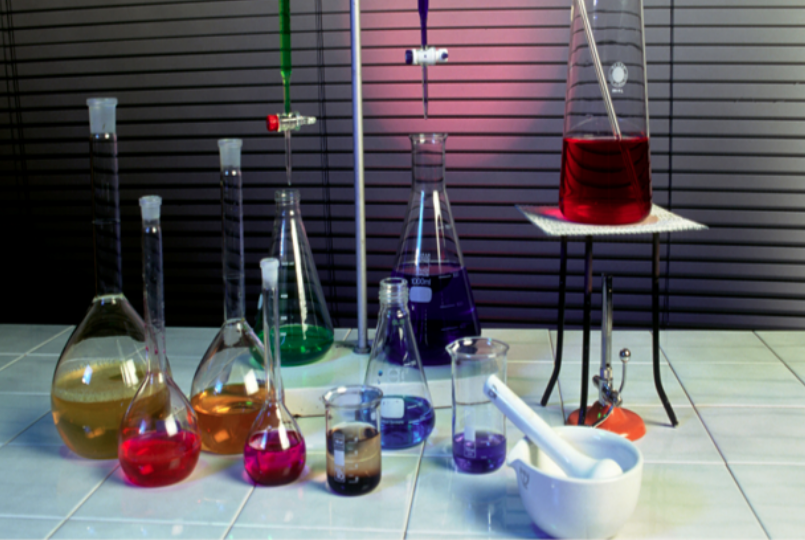
\includegraphics[width = \textwidth]{uibposter-images/bilde1.png}
    %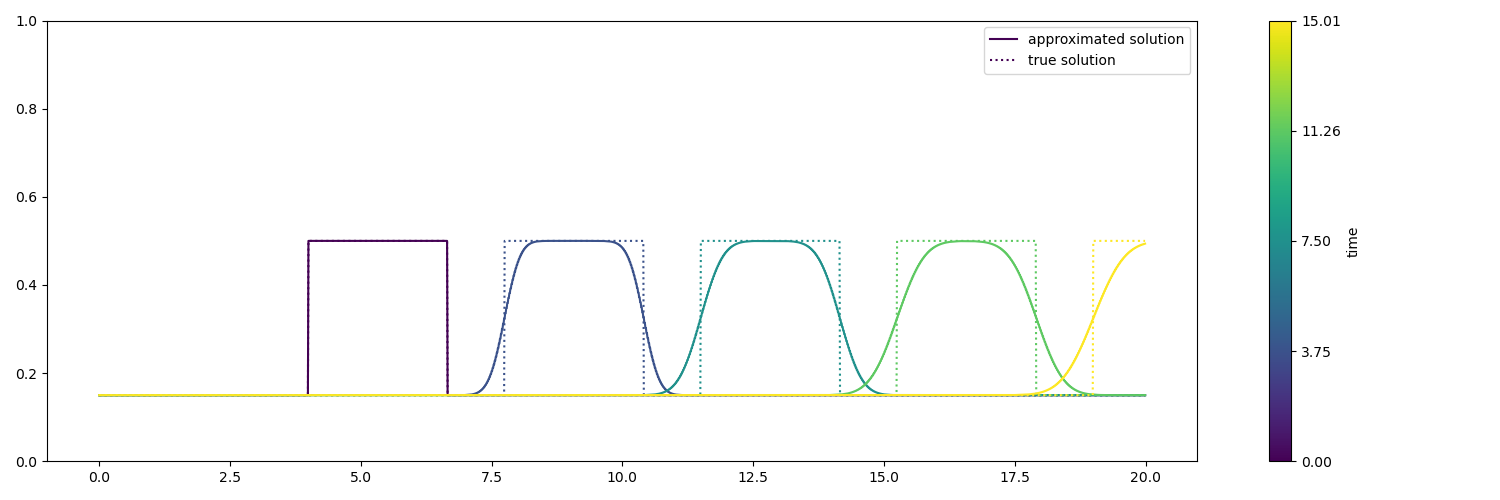
\includegraphics[width=0.95\textwidth, axisratio=7/3]{uibposter-images/test1.tikz}
    \begin{figure}[h]
    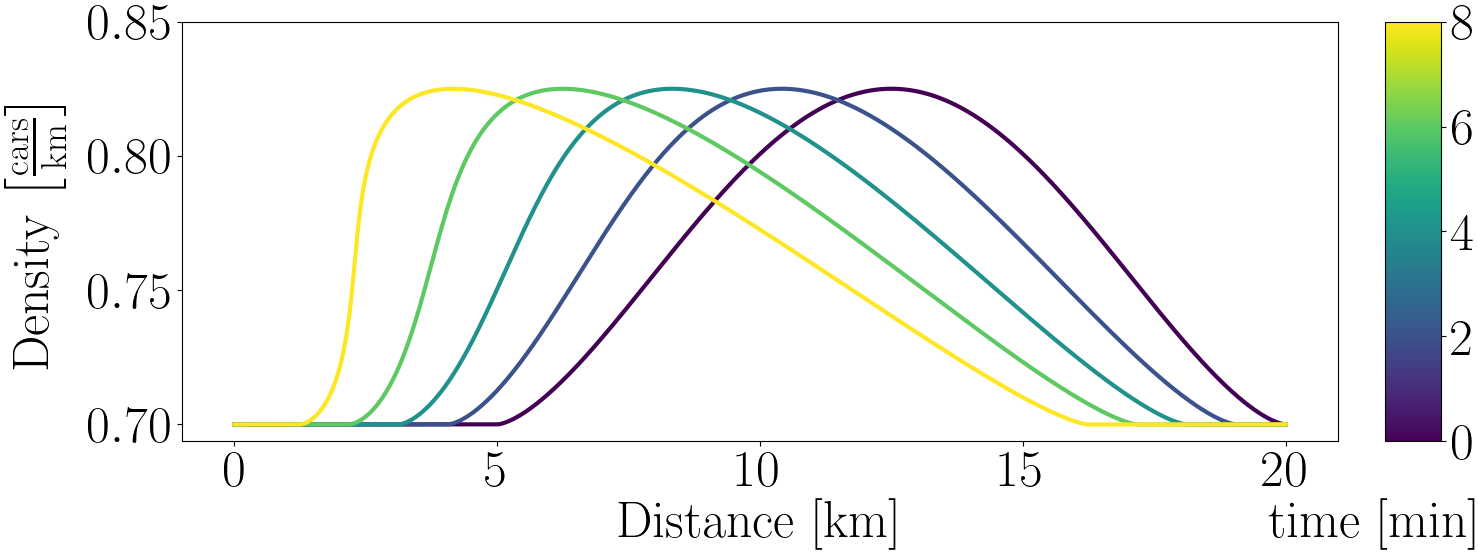
\includegraphics[width=\textwidth]{fig/traffic_motivation_laxW_continous.png} \caption{Build up of a traffic jam produced by the braking of some cars.} \label{img:traffic_flow_motivation}	
    \end{figure}
    \vspace{0.5cm}

\begin{column}{0.5\textwidth - 1.5cm}
\textbf{Abstract}
\vspace{0.5cm}

{\fontsize{40}{15}\selectfont
	We present the Lax-Wendroff method for hyperbolic conservation laws. Based on the one-dimensional case we illustrate how the scheme works and compare it with other numerical methods. This leads us to the conclusion that the Lax-Wendroff scheme is superior to the currently used methods.}

\vspace{0.5cm}
\textbf{Introduction}
\vspace{0.5cm}

Hyperbolic conservation laws are time-dependent systems of PDE's describing the conservation of some quantities, such as mass, momentum or heat. The equation is given as:
\begin{align*}
    u_t + f(u)_x = 0
\end{align*}
Where $u(x,t)$ is the conserved quantity, while $f(u)$ is the flux function. Flux functions are commonly nonlinear, leading to nonlinear systems of PDEs where, in general, the exact solution is unknown. Hence numerical methods are used, to compute an approximation. 

\vspace{0.5cm}
This can be used to simulate traffic jams as illustrated in \cref{img:traffic_flow_motivation}. In this case cars are moving from left to right, but the traffic jam moves in the opposite direction. 

\vspace{0.5cm}
\textbf{The Lax-Wendroff Method}

\vspace{0.5cm}
The method can be seen as a concatenation of the Lax-Friderich scheme.
The general formula is given by:
\begin{align*}
&U_j^{n+1} = U_j^n\\
&- \frac{k}{h}\left(f\left(U_{j+\frac{1}{2}}^{n+\frac{1}{2}}\right) - f\left(U_{j-\frac{1}{2}}^{n+\frac{1}{2}}\right)\right)
\end{align*}

\end{column}
\begin{column}{0.5\textwidth - 1.5cm}
where $k$ stepsize in time, $h$ stepsize in space and
\begin{align*}
U_{j+\frac{1}{2}}^{n+\frac{1}{2}} =&~ \frac{1}{2} (U_j^n + U_{j+1}^n)\\
&- \frac{k}{2h}[f(U_{j+1}^n) - f(U_j^n)].
\end{align*}
As known from the first order schemes, the step size has to be chosen in a fixed ratio. This fact is motivated by the CFL condition of the linear case ($u_t + au_x = 0$), where we need $|\nu| = \frac{k}{h} |a| < 1$. 
%The computation of the next time step can be written as a function of the solution of the current timestep by $U^{n+1} = \mathcal{H}(U^n)$. This notation can be used to define the local truncation error of a method by
%\begin{align*}
%L_k(x, t) = \frac{u(x, t+k) - \mathcal{H}(u(\cdot, t); x)}{k}
%\end{align*}
%contingent on the used step size in time $k$. This error will now be considered in the linear advection equation with $a > 0$. By Taylor expansion around $u(x, t)$ and some simplifications this yields to:

\vspace{0.5cm}
Computing the local truncation error of Lax-Wendroff yields
\begin{align*}
L_k(x, t) = &\frac{a}{6}(a^2 k^2 - h^2)u_{xxx} \\
&+ \mathcal{O}(h^3) \text{,}
\end{align*}
therefore it is a consistent second order method. 
%Additional for stability the condition $|\nu| < 1$ where $\nu = a\frac{k}{h}$ is the Courant number must be fulfilled. 
In the case of a linear advection equation the convergence of a method follows from consistency and stability by the Lax equivalence theorem. For the nonlinear case it is proven that a consistent numerical method with bounded solutions always converges to a weak solution of the equation.

\vspace{0.5cm}
The local truncation error also leads to the modified equation which is given as:
\begin{align*}
u_t + a u_x &= \frac{a}{6} (a^2 k^2 - h^2) u_{xxx}\\
&:= \mu u_{xxx}
\end{align*}

This is also a dispersive equation and a solution $u(x, t)$ of it can be represented in Fourier space. Isolating each wavenumber $\xi$ by applying solutions of the form $u(x,t) = e^{i(\xi x - c(\xi)t)}$ to the linear advection equation yields the dispersion relation:
\begin{align*}
c(\xi) = a\xi + \mu \xi^3
\end{align*}

    \end{column}
\end{column}
\begin{column}{0.5\textwidth - 1.5cm}
\begin{column}{0.5\textwidth - 1.5cm}
\vspace*{-2cm}

Based on this relation its possible to calculate the group velocity $c’(\xi)$ for wavenumber $\xi$ which describes in which speed a wave peak travel. It is given by:
\begin{align*}
c'(\xi) = a + 3\mu \xi^2
\end{align*}
As $\mu = \frac{a}{6}h^2(\nu^2 - 1)$ and since, without loss of generality, $a > 0$ and for stability $|\nu| < 1$ the group velocity $c’(\xi)$ is smaller than $a$ for all $\xi$, but tends to $a$ as $h\rightarrow0$. It follows that the scheme leads to an oscillatory wave train lagging behind the discontinuity, which is traveling with speed $a$. This can also be seen later in the numerical experiments.
    
\vspace{0.5cm}
\textbf{Numerical Analysis}
\vspace{0.5cm}
    
Applying the method to problems with discontinuous initial data illustrates the properties of the scheme.

\vspace{0.5cm}
For the linear advection equation this gives the approximations shown in \cref{img:linar_comprehension}. 
As commented before the Lax-Wendroff scheme oscillates in front of the discontinuity of the true solution. However, the discontinuity is approximated more accurate what leads to a smaller error which is shown in \cref{img:error_over_time}. Also notice that Lax-Friedrichs looses height over time. 

\begin{figure}[h]
	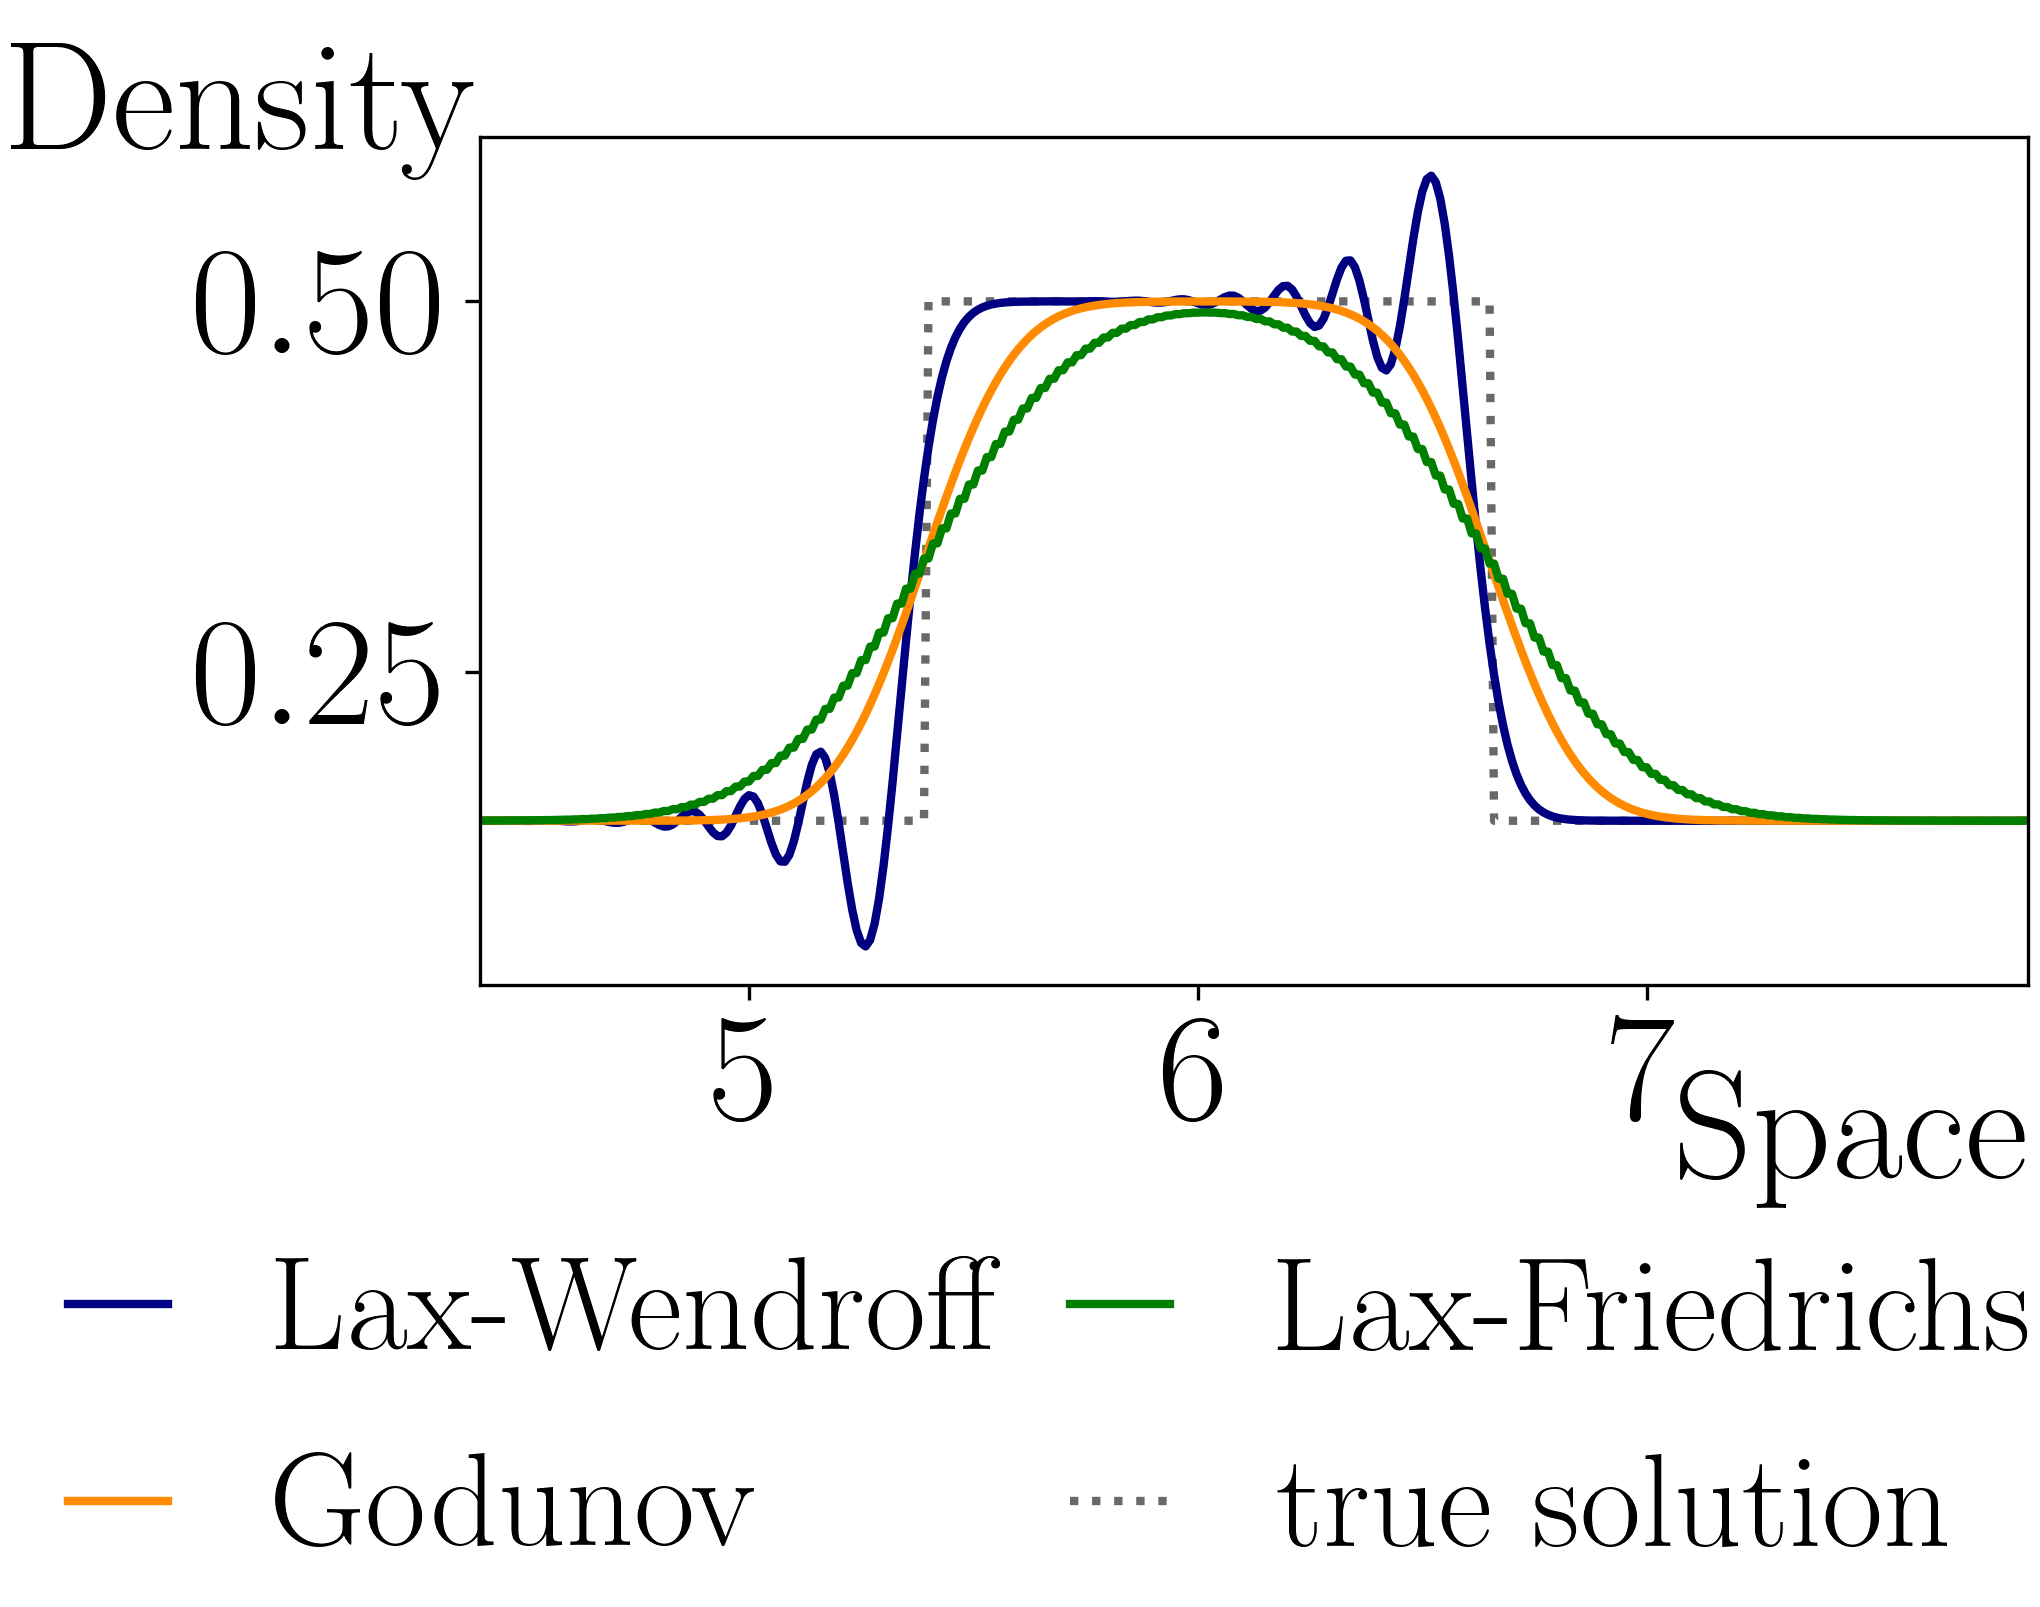
\includegraphics{fig/linear_compare.png}
	\caption{Approximations for the linear advection equation at time $t = 5$.}
	\label{img:linar_comprehension}
\end{figure}

%\vspace{0.5cm}
Comparing the runtime of the methods to compute \cref{img:linar_comprehension} it turns out that the Godunov's one is by far the slowest which is due to its non-vectorized standard form.
Looking deeper into \cref{img:error_over_time} we can confirm that the Lax-Wendroff method has the lowest error as expected due to its higher order.

\end{column}
\begin{column}{0.5\textwidth - 1.5cm}
	\vspace*{-1.7cm} 

   
    \begin{figure}
    	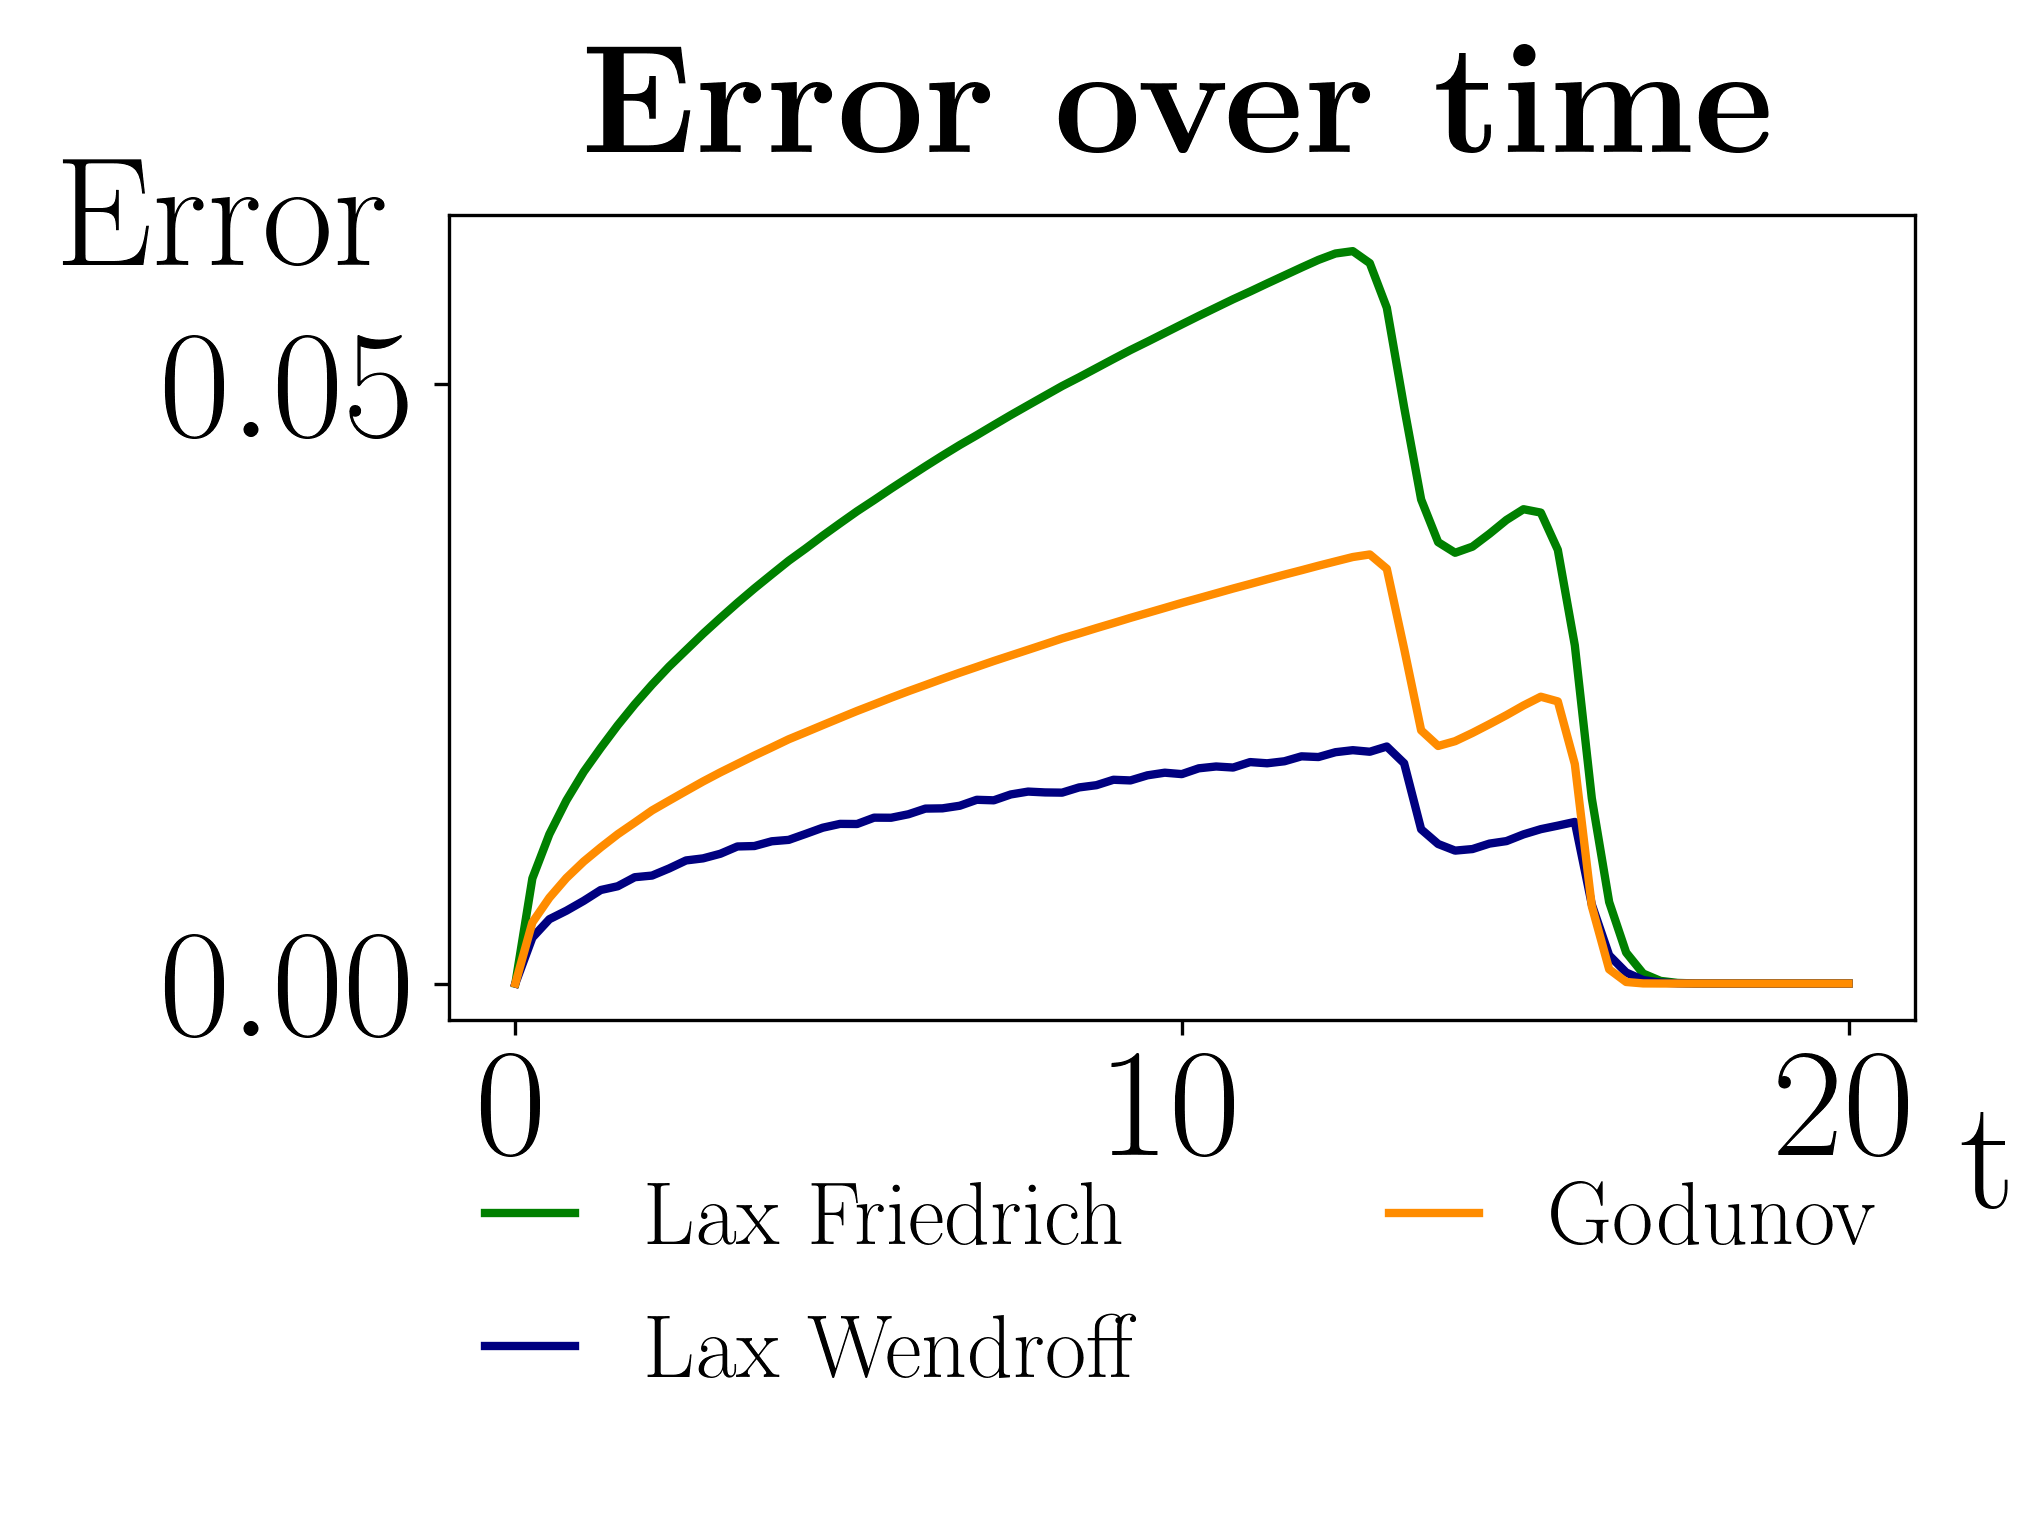
\includegraphics{fig/error_over_time.png}
    	\caption{Error of the considered scheme over time for the problem used in \cref{img:linar_comprehension}.}
    	\label{img:error_over_time}
    \end{figure}

Looking at the Burger's, the traffic and the Buckley-Leverett equation in \cref{img:non_lin_equation}, the obtained result is still quite accurate and we can see similar behavior. Note again the predicted oscillations of Lax-Wendroff in front of to the discontinuity.

\begin{figure}
	\begin{subfigure}{\textwidth}
	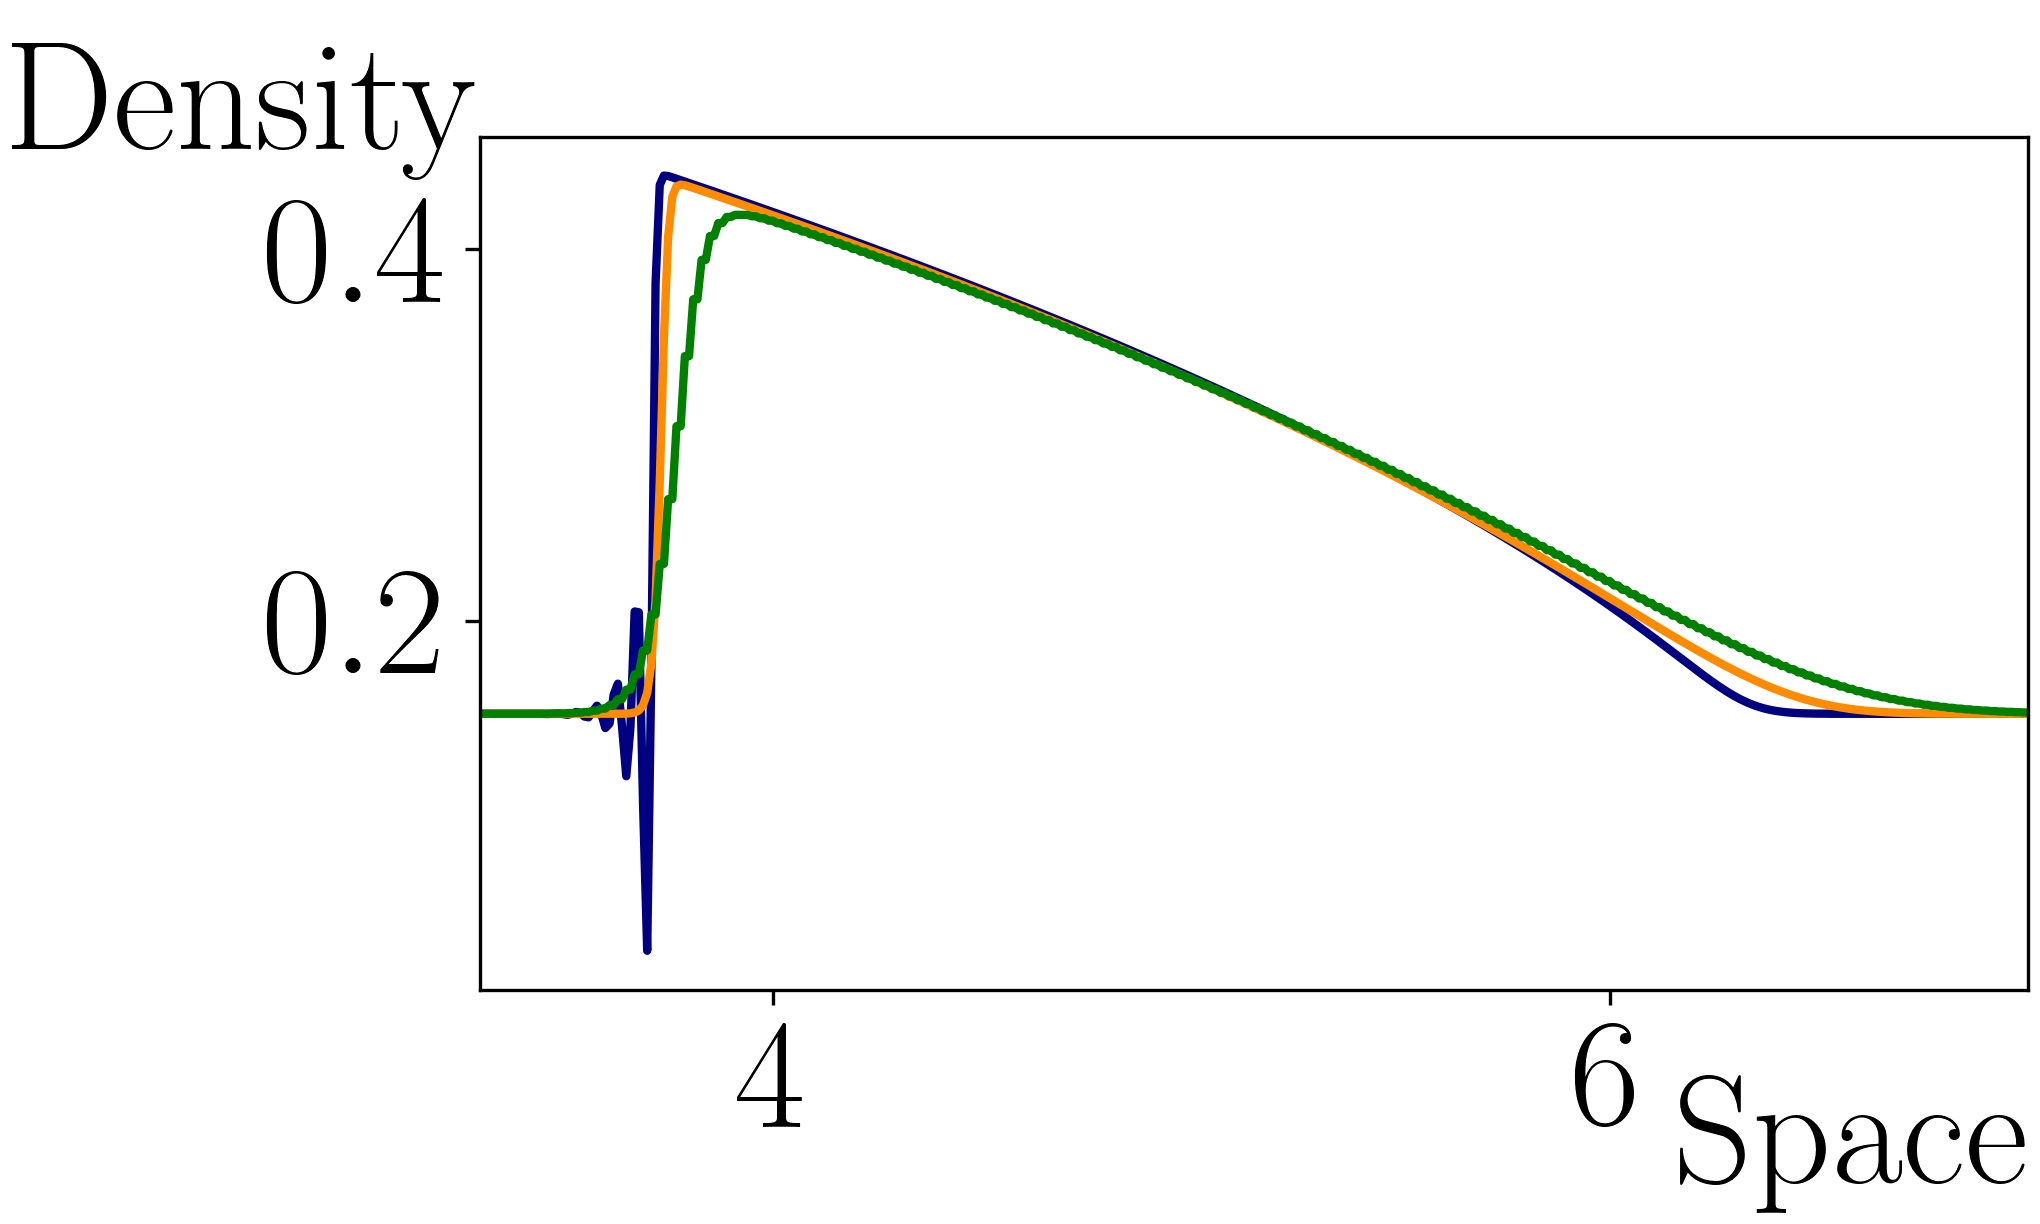
\includegraphics{fig/traffic_compare_.png}
	\end{subfigure}

	\begin{subfigure}{\textwidth}
		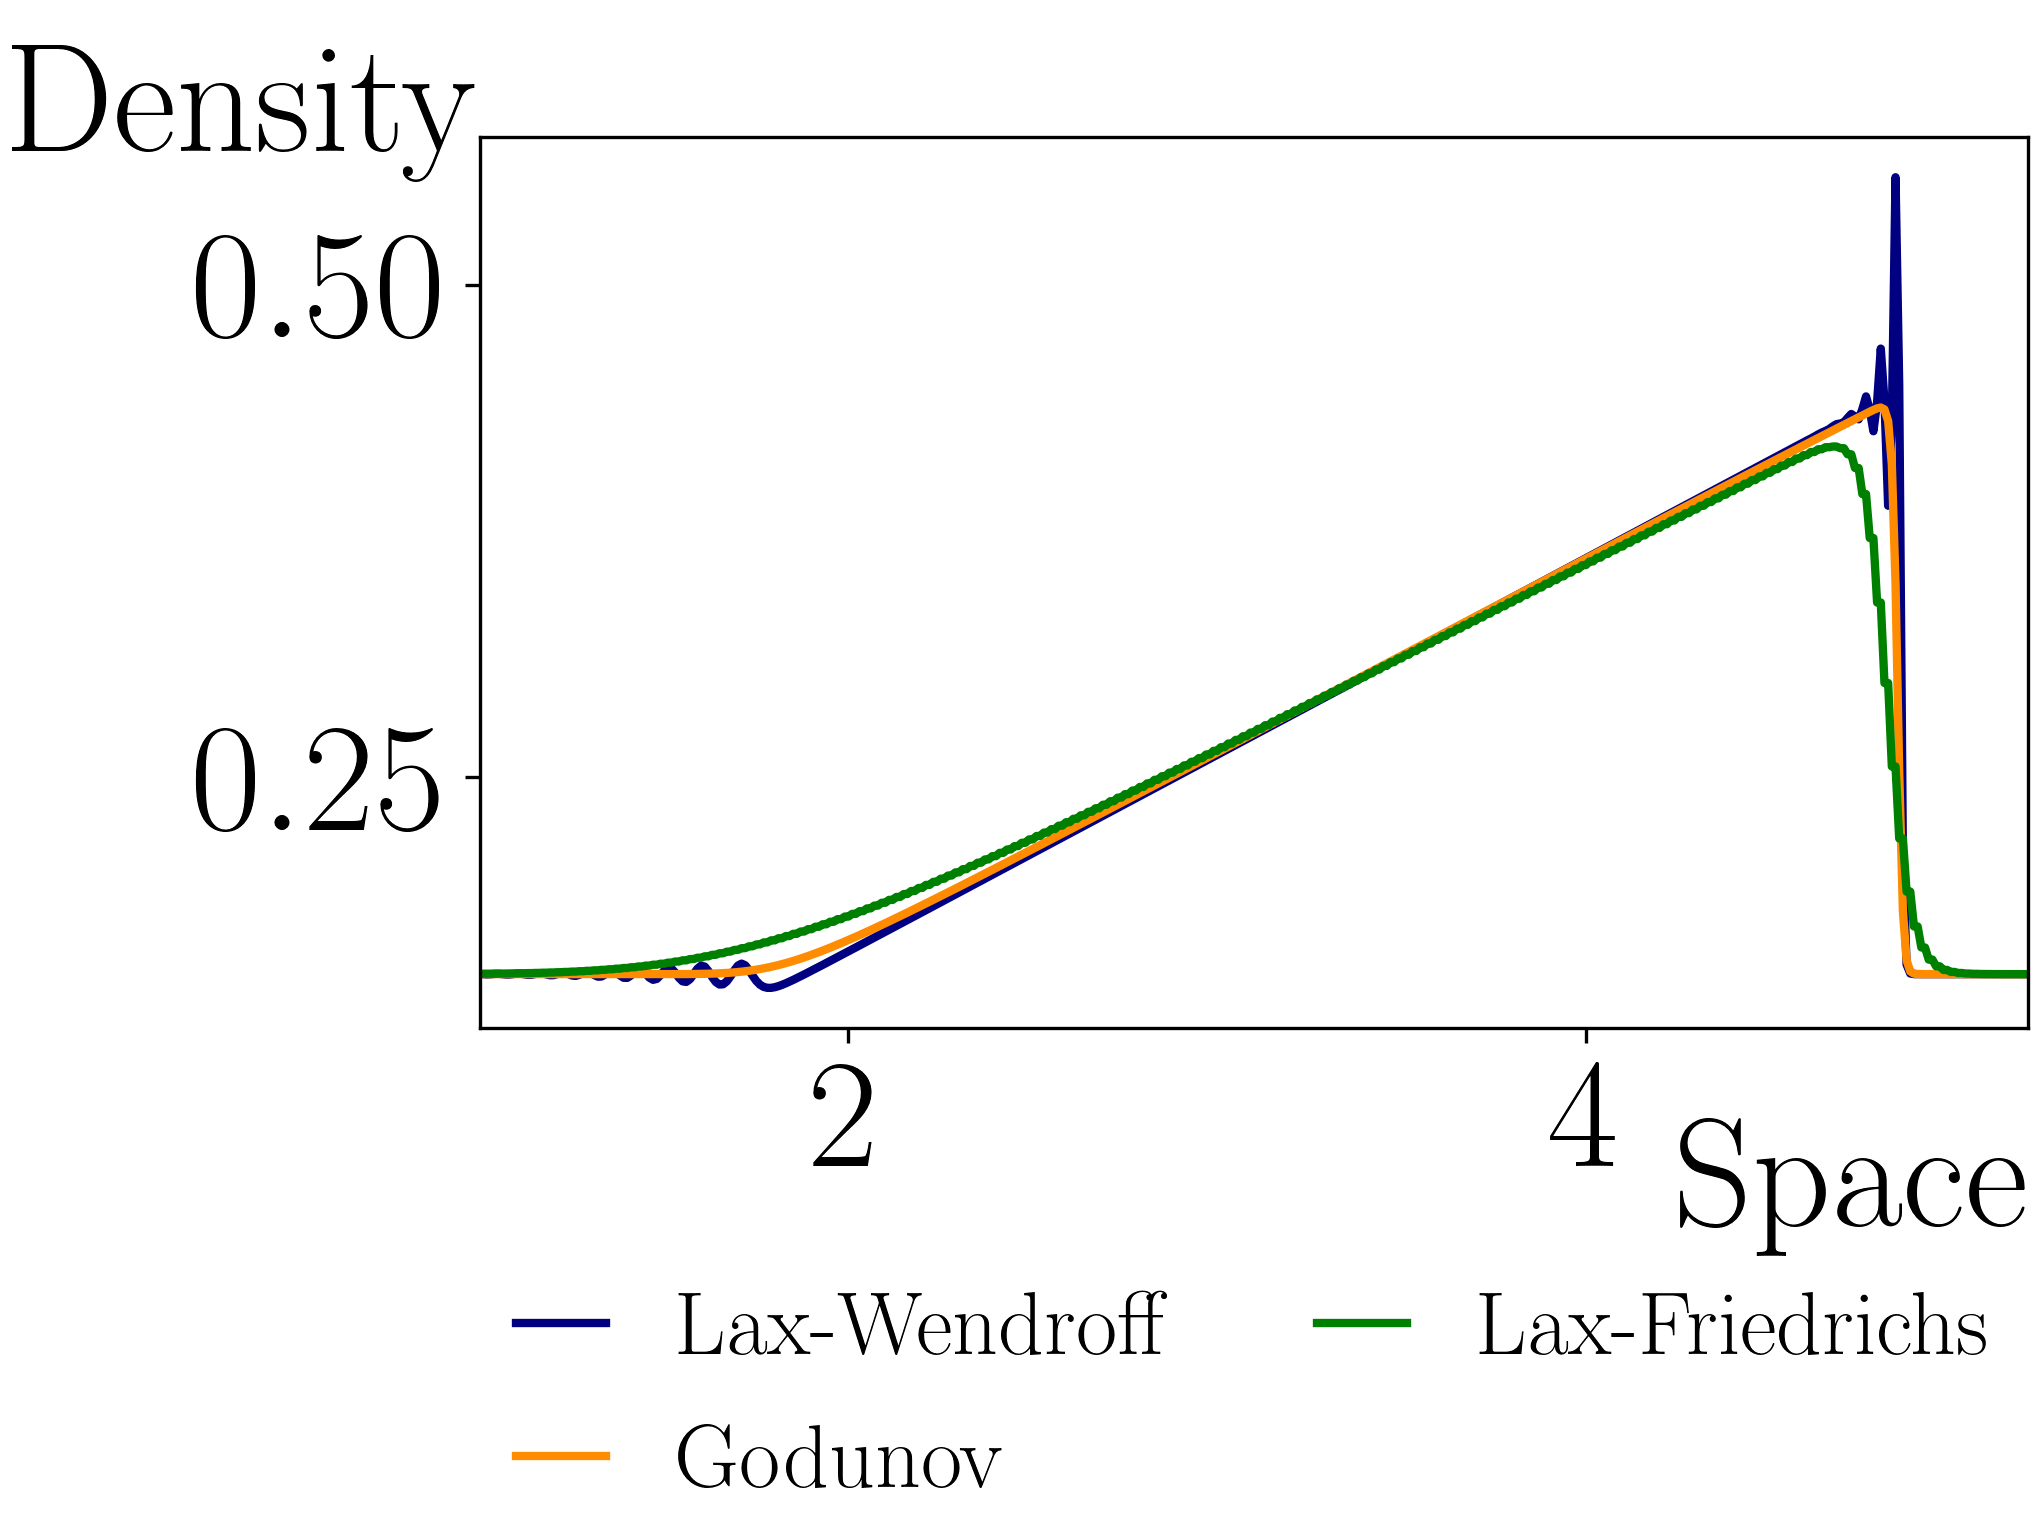
\includegraphics{fig/burger_compare.png}
	\end{subfigure}

	\begin{subfigure}{\textwidth}
		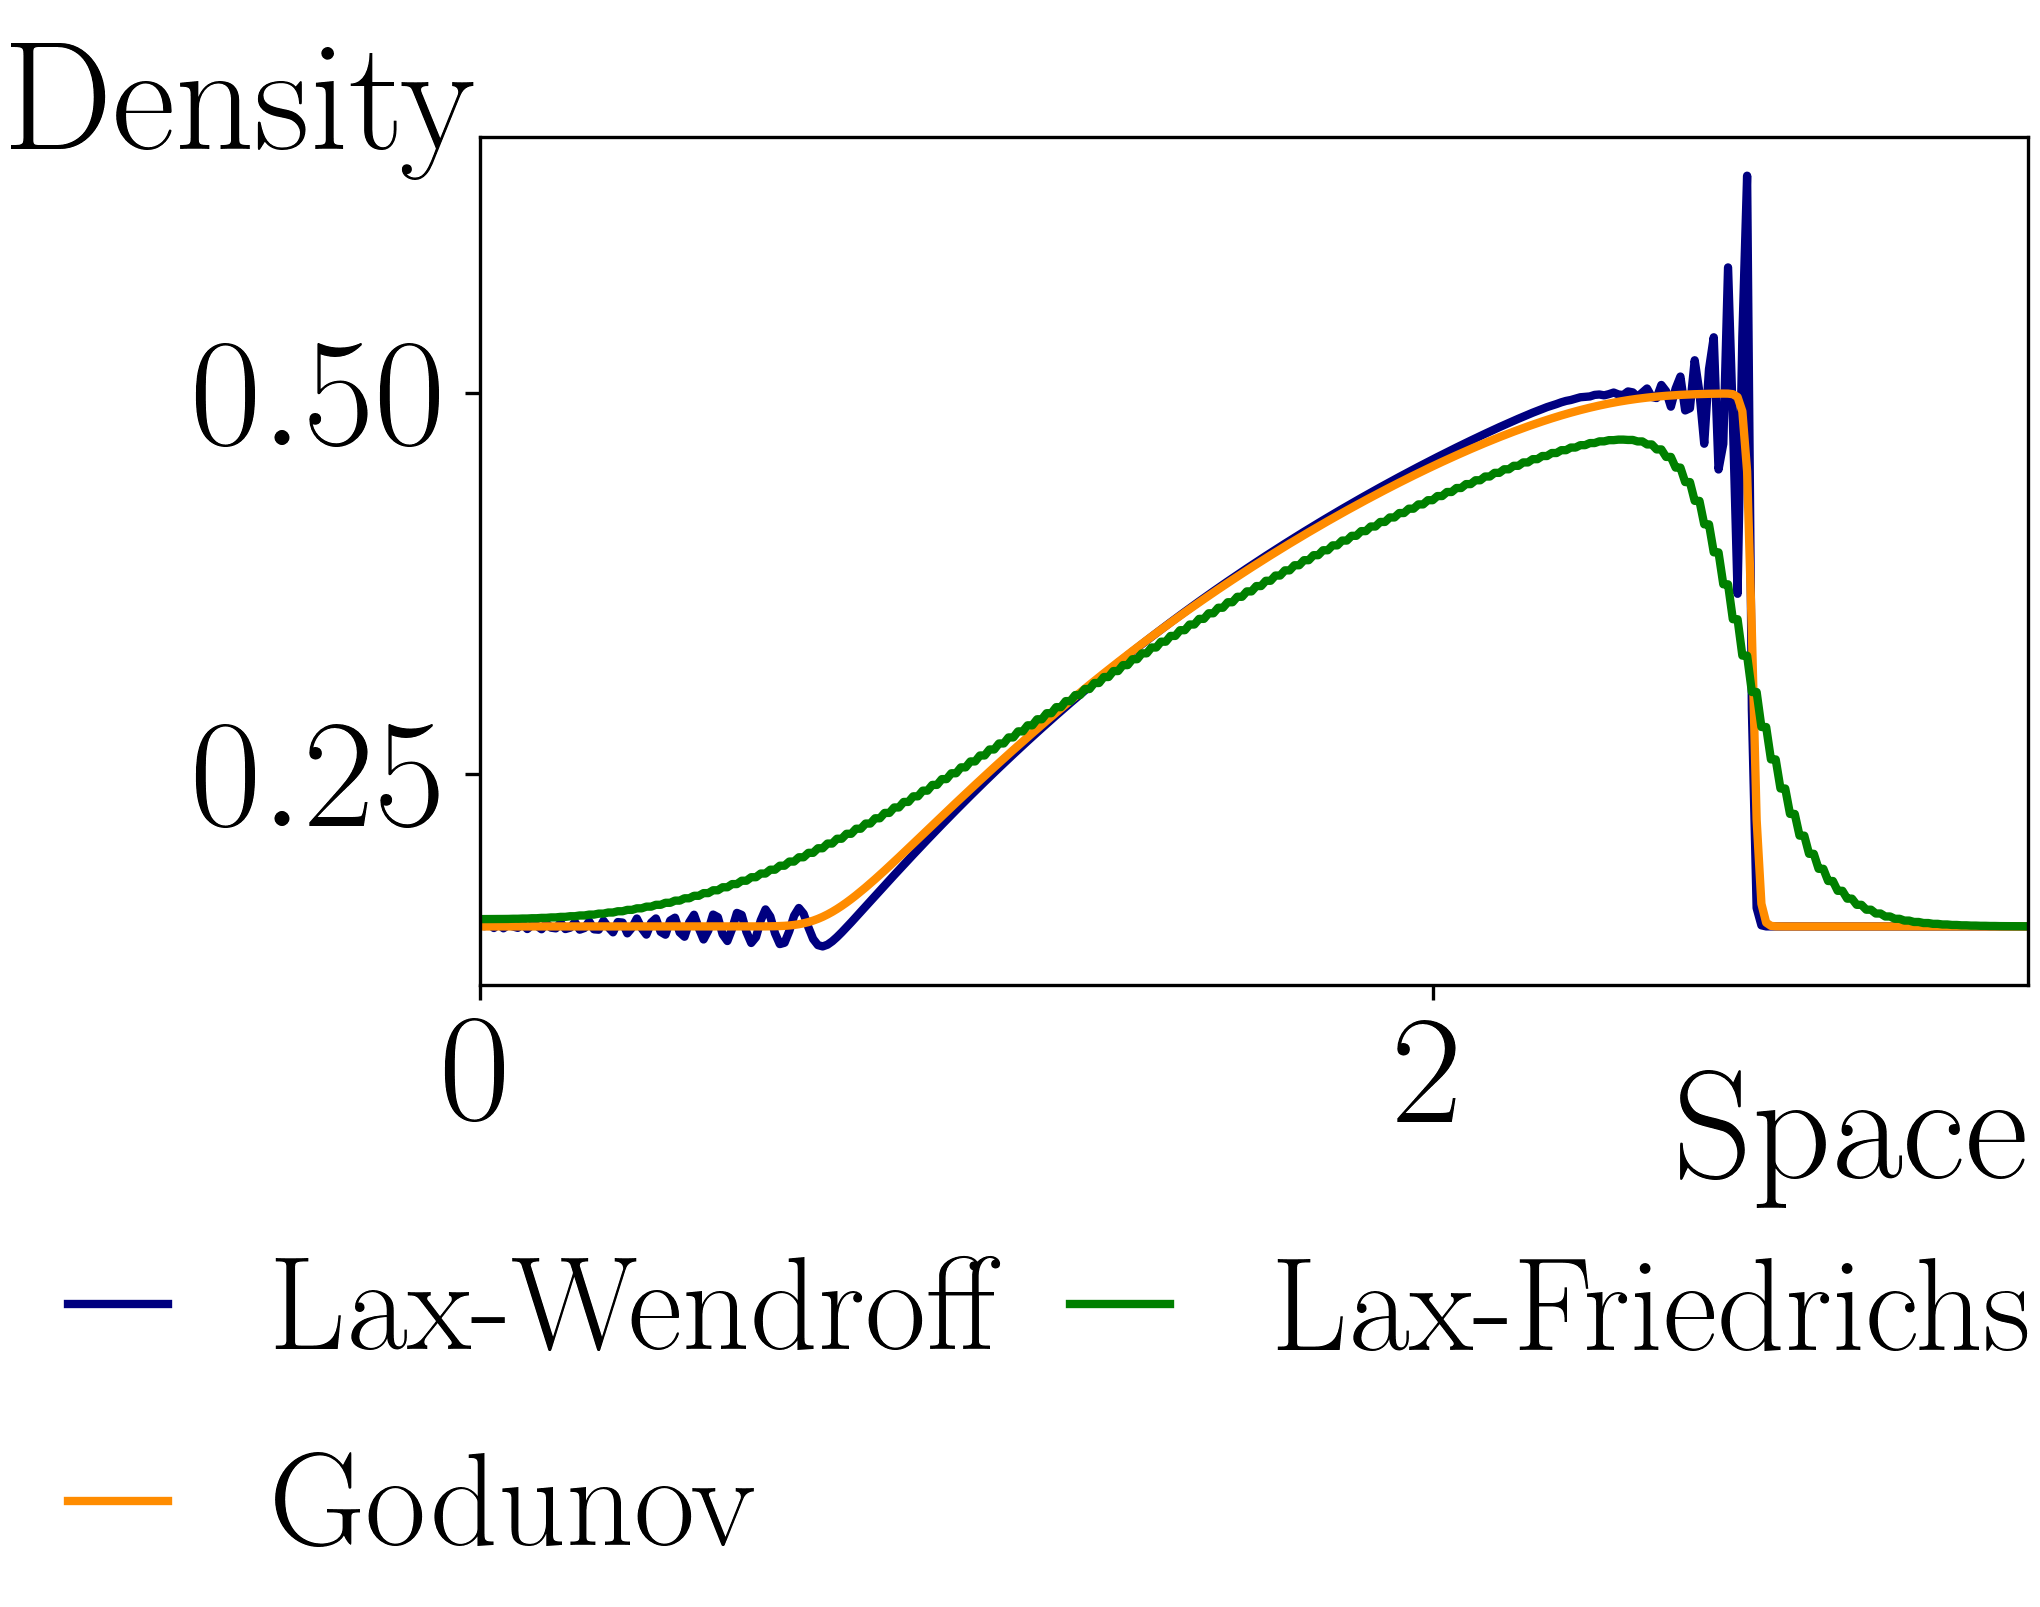
\includegraphics{fig/buckley_compare.png}
	\end{subfigure}
	\caption{Approximations for the traffic equation (top), the Burger's equation (middle) and the Buckley-Leverett equation (bottom) at time $t = 5$.}
	\label{img:non_lin_equation}
\end{figure}

\textbf{Conclusion}

\vspace{0.5cm}
With the Lax-Wendroff method it is possible to get accurate approximations of a discontinuity in short runtime. 
%So we can conclude that the it can compete even with the Godunov one.
This makes it a serious competitor to the Godunov scheme.
%, which is very used nowadays.

    \vspace{0.5cm}
    \textbf{\scriptsize{References}}
    \vspace{0.3cm}
    \nocite{*}
    \bibliographystyle{apacite}
    \bibliography{references}
    

\end{column}
\end{column}
\end{columns}





\end{frame}
\end{document}